\documentclass[1p]{elsarticle_modified}
%\bibliographystyle{elsarticle-num}

%\usepackage[colorlinks]{hyperref}
%\usepackage{abbrmath_seonhwa} %\Abb, \Ascr, \Acal ,\Abf, \Afrak
\usepackage{amsfonts}
\usepackage{amssymb}
\usepackage{amsmath}
\usepackage{amsthm}
\usepackage{scalefnt}
\usepackage{amsbsy}
\usepackage{kotex}
\usepackage{caption}
\usepackage{subfig}
\usepackage{color}
\usepackage{graphicx}
\usepackage{xcolor} %% white, black, red, green, blue, cyan, magenta, yellow
\usepackage{float}
\usepackage{setspace}
\usepackage{hyperref}

\usepackage{tikz}
\usetikzlibrary{arrows}

\usepackage{multirow}
\usepackage{array} % fixed length table
\usepackage{hhline}

%%%%%%%%%%%%%%%%%%%%%
\makeatletter
\renewcommand*\env@matrix[1][\arraystretch]{%
	\edef\arraystretch{#1}%
	\hskip -\arraycolsep
	\let\@ifnextchar\new@ifnextchar
	\array{*\c@MaxMatrixCols c}}
\makeatother %https://tex.stackexchange.com/questions/14071/how-can-i-increase-the-line-spacing-in-a-matrix
%%%%%%%%%%%%%%%

\usepackage[normalem]{ulem}

\newcommand{\msout}[1]{\ifmmode\text{\sout{\ensuremath{#1}}}\else\sout{#1}\fi}
%SOURCE: \msout is \stkout macro in https://tex.stackexchange.com/questions/20609/strikeout-in-math-mode

\newcommand{\cancel}[1]{
	\ifmmode
	{\color{red}\msout{#1}}
	\else
	{\color{red}\sout{#1}}
	\fi
}

\newcommand{\add}[1]{
	{\color{blue}\uwave{#1}}
}

\newcommand{\replace}[2]{
	\ifmmode
	{\color{red}\msout{#1}}{\color{blue}\uwave{#2}}
	\else
	{\color{red}\sout{#1}}{\color{blue}\uwave{#2}}
	\fi
}

\newcommand{\Sol}{\mathcal{S}} %segment
\newcommand{\D}{D} %diagram
\newcommand{\A}{\mathcal{A}} %arc


%%%%%%%%%%%%%%%%%%%%%%%%%%%%%5 test

\def\sl{\operatorname{\textup{SL}}(2,\Cbb)}
\def\psl{\operatorname{\textup{PSL}}(2,\Cbb)}
\def\quan{\mkern 1mu \triangleright \mkern 1mu}

\theoremstyle{definition}
\newtheorem{thm}{Theorem}[section]
\newtheorem{prop}[thm]{Proposition}
\newtheorem{lem}[thm]{Lemma}
\newtheorem{ques}[thm]{Question}
\newtheorem{cor}[thm]{Corollary}
\newtheorem{defn}[thm]{Definition}
\newtheorem{exam}[thm]{Example}
\newtheorem{rmk}[thm]{Remark}
\newtheorem{alg}[thm]{Algorithm}

\newcommand{\I}{\sqrt{-1}}
\begin{document}

%\begin{frontmatter}
%
%\title{Boundary parabolic representations of knots up to 8 crossings}
%
%%% Group authors per affiliation:
%\author{Yunhi Cho} 
%\address{Department of Mathematics, University of Seoul, Seoul, Korea}
%\ead{yhcho@uos.ac.kr}
%
%
%\author{Seonhwa Kim} %\fnref{s_kim}}
%\address{Center for Geometry and Physics, Institute for Basic Science, Pohang, 37673, Korea}
%\ead{ryeona17@ibs.re.kr}
%
%\author{Hyuk Kim}
%\address{Department of Mathematical Sciences, Seoul National University, Seoul 08826, Korea}
%\ead{hyukkim@snu.ac.kr}
%
%\author{Seokbeom Yoon}
%\address{Department of Mathematical Sciences, Seoul National University, Seoul, 08826,  Korea}
%\ead{sbyoon15@snu.ac.kr}
%
%\begin{abstract}
%We find all boundary parabolic representation of knots up to 8 crossings.
%
%\end{abstract}
%\begin{keyword}
%    \MSC[2010] 57M25 
%\end{keyword}
%
%\end{frontmatter}

%\linenumbers
%\tableofcontents
%
\newcommand\colored[1]{\textcolor{white}{\rule[-0.35ex]{0.8em}{1.4ex}}\kern-0.8em\color{red} #1}%
%\newcommand\colored[1]{\textcolor{white}{ #1}\kern-2.17ex	\textcolor{white}{ #1}\kern-1.81ex	\textcolor{white}{ #1}\kern-2.15ex\color{red}#1	}

{\Large $\underline{12n_{0565}~(K12n_{0565})}$}

\setlength{\tabcolsep}{10pt}
\renewcommand{\arraystretch}{1.6}
\vspace{1cm}\begin{tabular}{m{100pt}>{\centering\arraybackslash}m{274pt}}
\multirow{5}{120pt}{
	\centering
	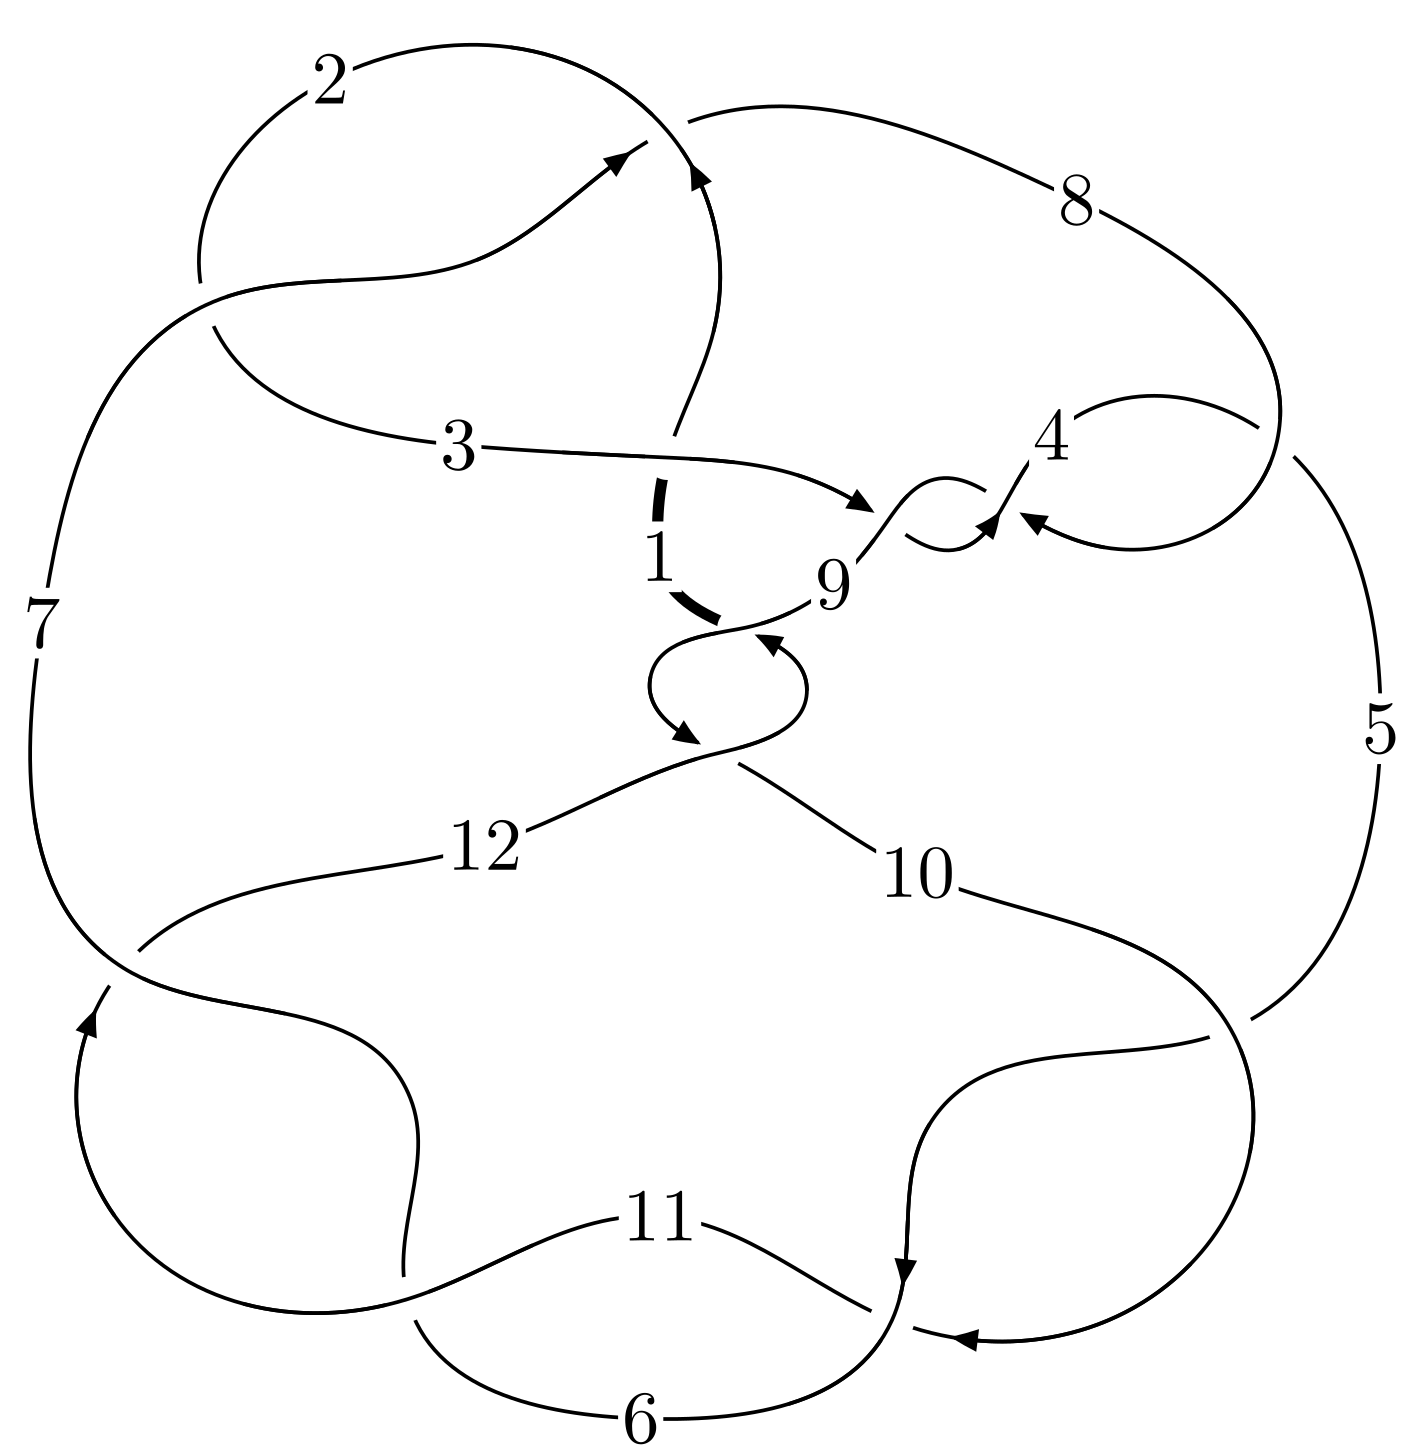
\includegraphics[width=112pt]{../../../GIT/diagram.site/Diagrams/png/2654_12n_0565.png}\\
\ \ \ A knot diagram\footnotemark}&
\allowdisplaybreaks
\textbf{Linearized knot diagam} \\
\cline{2-2}
 &
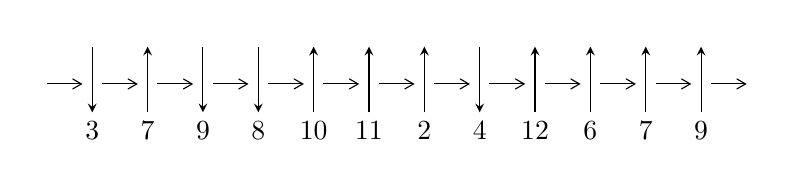
\begin{tikzpicture}[x=20pt, y=17pt]
	% nodes
	\node (C0) at (0, 0) {};
	\node (C1) at (1, 0) {};
	\node (C1U) at (1, +1) {};
	\node (C1D) at (1, -1) {3};

	\node (C2) at (2, 0) {};
	\node (C2U) at (2, +1) {};
	\node (C2D) at (2, -1) {7};

	\node (C3) at (3, 0) {};
	\node (C3U) at (3, +1) {};
	\node (C3D) at (3, -1) {9};

	\node (C4) at (4, 0) {};
	\node (C4U) at (4, +1) {};
	\node (C4D) at (4, -1) {8};

	\node (C5) at (5, 0) {};
	\node (C5U) at (5, +1) {};
	\node (C5D) at (5, -1) {10};

	\node (C6) at (6, 0) {};
	\node (C6U) at (6, +1) {};
	\node (C6D) at (6, -1) {11};

	\node (C7) at (7, 0) {};
	\node (C7U) at (7, +1) {};
	\node (C7D) at (7, -1) {2};

	\node (C8) at (8, 0) {};
	\node (C8U) at (8, +1) {};
	\node (C8D) at (8, -1) {4};

	\node (C9) at (9, 0) {};
	\node (C9U) at (9, +1) {};
	\node (C9D) at (9, -1) {12};

	\node (C10) at (10, 0) {};
	\node (C10U) at (10, +1) {};
	\node (C10D) at (10, -1) {6};

	\node (C11) at (11, 0) {};
	\node (C11U) at (11, +1) {};
	\node (C11D) at (11, -1) {7};

	\node (C12) at (12, 0) {};
	\node (C12U) at (12, +1) {};
	\node (C12D) at (12, -1) {9};
	\node (C13) at (13, 0) {};

	% arrows
	\draw[->,>={angle 60}]
	(C0) edge (C1) (C1) edge (C2) (C2) edge (C3) (C3) edge (C4) (C4) edge (C5) (C5) edge (C6) (C6) edge (C7) (C7) edge (C8) (C8) edge (C9) (C9) edge (C10) (C10) edge (C11) (C11) edge (C12) (C12) edge (C13) ;	\draw[->,>=stealth]
	(C1U) edge (C1D) (C2D) edge (C2U) (C3U) edge (C3D) (C4U) edge (C4D) (C5D) edge (C5U) (C6D) edge (C6U) (C7D) edge (C7U) (C8U) edge (C8D) (C9D) edge (C9U) (C10D) edge (C10U) (C11D) edge (C11U) (C12D) edge (C12U) ;
	\end{tikzpicture} \\
\hhline{~~} \\& 
\textbf{Solving Sequence} \\ \cline{2-2} 
 &
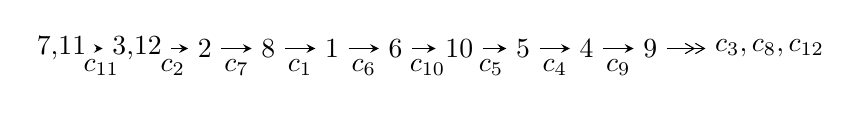
\begin{tikzpicture}[x=23pt, y=7pt]
	% node
	\node (A0) at (-1/8, 0) {7,11};
	\node (A1) at (17/16, 0) {3,12};
	\node (A2) at (17/8, 0) {2};
	\node (A3) at (25/8, 0) {8};
	\node (A4) at (33/8, 0) {1};
	\node (A5) at (41/8, 0) {6};
	\node (A6) at (49/8, 0) {10};
	\node (A7) at (57/8, 0) {5};
	\node (A8) at (65/8, 0) {4};
	\node (A9) at (73/8, 0) {9};
	\node (C1) at (1/2, -1) {$c_{11}$};
	\node (C2) at (13/8, -1) {$c_{2}$};
	\node (C3) at (21/8, -1) {$c_{7}$};
	\node (C4) at (29/8, -1) {$c_{1}$};
	\node (C5) at (37/8, -1) {$c_{6}$};
	\node (C6) at (45/8, -1) {$c_{10}$};
	\node (C7) at (53/8, -1) {$c_{5}$};
	\node (C8) at (61/8, -1) {$c_{4}$};
	\node (C9) at (69/8, -1) {$c_{9}$};
	\node (A10) at (11, 0) {$c_{3},c_{8},c_{12}$};

	% edge
	\draw[->,>=stealth]	
	(A0) edge (A1) (A1) edge (A2) (A2) edge (A3) (A3) edge (A4) (A4) edge (A5) (A5) edge (A6) (A6) edge (A7) (A7) edge (A8) (A8) edge (A9) ;
	\draw[->>,>={angle 60}]	
	(A9) edge (A10);
\end{tikzpicture} \\ 

\end{tabular} \\

\footnotetext{
The image of knot diagram is generated by the software ``\textbf{Draw programme}" developed by Andrew Bartholomew(\url{http://www.layer8.co.uk/maths/draw/index.htm\#Running-draw}), where we modified some parts for our purpose(\url{https://github.com/CATsTAILs/LinksPainter}).
}\phantom \\ \newline 
\centering \textbf{Ideals for irreducible components\footnotemark of $X_{\text{par}}$} 
 
\begin{align*}
I^u_{1}&=\langle 
5 u^{23}-65 u^{21}+\cdots+4 b+8,\;- u^{23}+14 u^{21}+\cdots+4 a-4,\;u^{24}+2 u^{23}+\cdots- u+2\rangle \\
I^u_{2}&=\langle 
- u^6+u^5+3 u^4-3 u^3-2 u^2+b+u,\;u^6-4 u^4+4 u^2+a,\;u^8-5 u^6+7 u^4-2 u^2+1\rangle \\
I^u_{3}&=\langle 
a^2 u+a^2+2 a u+b+2 a,\;a^3- a u+2 a+u-2,\;u^2- u-1\rangle \\
\\
\end{align*}
\raggedright * 3 irreducible components of $\dim_{\mathbb{C}}=0$, with total 38 representations.\\
\footnotetext{All coefficients of polynomials are rational numbers. But the coefficients are sometimes approximated in decimal forms when there is not enough margin.}
\newpage
\renewcommand{\arraystretch}{1}
\centering \section*{I. $I^u_{1}= \langle 5 u^{23}-65 u^{21}+\cdots+4 b+8,\;- u^{23}+14 u^{21}+\cdots+4 a-4,\;u^{24}+2 u^{23}+\cdots- u+2 \rangle$}
\flushleft \textbf{(i) Arc colorings}\\
\begin{tabular}{m{7pt} m{180pt} m{7pt} m{180pt} }
\flushright $a_{7}=$&$\begin{pmatrix}0\\u\end{pmatrix}$ \\
\flushright $a_{11}=$&$\begin{pmatrix}1\\0\end{pmatrix}$ \\
\flushright $a_{3}=$&$\begin{pmatrix}\frac{1}{4} u^{23}-\frac{7}{2} u^{21}+\cdots+\frac{1}{4} u+1\\-\frac{5}{4} u^{23}+\frac{65}{4} u^{21}+\cdots+\frac{5}{2} u-2\end{pmatrix}$ \\
\flushright $a_{12}=$&$\begin{pmatrix}1\\- u^2\end{pmatrix}$ \\
\flushright $a_{2}=$&$\begin{pmatrix}\frac{1}{4} u^{23}-\frac{7}{2} u^{21}+\cdots+\frac{1}{4} u+1\\-\frac{3}{4} u^{23}+\frac{39}{4} u^{21}+\cdots+\frac{3}{2} u-1\end{pmatrix}$ \\
\flushright $a_{8}=$&$\begin{pmatrix}\frac{1}{4} u^{19}-\frac{11}{4} u^{17}+\cdots+\frac{3}{4} u-1\\-\frac{1}{4} u^{21}+\frac{11}{4} u^{19}+\cdots-\frac{1}{2} u^2+\frac{1}{2} u\end{pmatrix}$ \\
\flushright $a_{1}=$&$\begin{pmatrix}u^8-5 u^6+7 u^4-2 u^2+1\\- u^{10}+4 u^8-3 u^6-2 u^4- u^2\end{pmatrix}$ \\
\flushright $a_{6}=$&$\begin{pmatrix}- u\\u\end{pmatrix}$ \\
\flushright $a_{10}=$&$\begin{pmatrix}- u^2+1\\u^2\end{pmatrix}$ \\
\flushright $a_{5}=$&$\begin{pmatrix}u^3-2 u\\- u^3+u\end{pmatrix}$ \\
\flushright $a_{4}=$&$\begin{pmatrix}\frac{1}{2} u^{13}-4 u^{11}+\cdots-\frac{3}{2} u+\frac{1}{2}\\-\frac{1}{4} u^{20}+\frac{11}{4} u^{18}+\cdots-\frac{5}{4} u^2+u\end{pmatrix}$ \\
\flushright $a_{9}=$&$\begin{pmatrix}u^4-3 u^2+1\\- u^6+2 u^4+u^2\end{pmatrix}$\\&\end{tabular}
\flushleft \textbf{(ii) Obstruction class $= -1$}\\~\\
\flushleft \textbf{(iii) Cusp Shapes $= 2 u^{23}-28 u^{21}+164 u^{19}+2 u^{18}-520 u^{17}-22 u^{16}+968 u^{15}+96 u^{14}-1076 u^{13}-210 u^{12}+672 u^{11}+242 u^{10}-116 u^9-148 u^8-170 u^7+50 u^6+116 u^5-2 u^4-38 u^3-2 u^2+6$}\\~\\
\newpage\renewcommand{\arraystretch}{1}
\flushleft \textbf{(iv) u-Polynomials at the component}\newline \\
\begin{tabular}{m{50pt}|m{274pt}}
Crossings & \hspace{64pt}u-Polynomials at each crossing \\
\hline $$\begin{aligned}c_{1}\end{aligned}$$&$\begin{aligned}
&u^{24}+u^{23}+\cdots-61 u+4
\end{aligned}$\\
\hline $$\begin{aligned}c_{2},c_{7}\end{aligned}$$&$\begin{aligned}
&u^{24}+u^{23}+\cdots+3 u+2
\end{aligned}$\\
\hline $$\begin{aligned}c_{3},c_{4},c_{8}\end{aligned}$$&$\begin{aligned}
&u^{24}+u^{23}+\cdots+9 u+2
\end{aligned}$\\
\hline $$\begin{aligned}c_{5},c_{6},c_{10}\\c_{11}\end{aligned}$$&$\begin{aligned}
&u^{24}-2 u^{23}+\cdots+u+2
\end{aligned}$\\
\hline $$\begin{aligned}c_{9},c_{12}\end{aligned}$$&$\begin{aligned}
&u^{24}+8 u^{23}+\cdots+5111 u+1016
\end{aligned}$\\
\hline
\end{tabular}\\~\\
\newpage\renewcommand{\arraystretch}{1}
\flushleft \textbf{(v) Riley Polynomials at the component}\newline \\
\begin{tabular}{m{50pt}|m{274pt}}
Crossings & \hspace{64pt}Riley Polynomials at each crossing \\
\hline $$\begin{aligned}c_{1}\end{aligned}$$&$\begin{aligned}
&y^{24}+53 y^{23}+\cdots-1345 y+16
\end{aligned}$\\
\hline $$\begin{aligned}c_{2},c_{7}\end{aligned}$$&$\begin{aligned}
&y^{24}+y^{23}+\cdots-61 y+4
\end{aligned}$\\
\hline $$\begin{aligned}c_{3},c_{4},c_{8}\end{aligned}$$&$\begin{aligned}
&y^{24}+37 y^{23}+\cdots-77 y+4
\end{aligned}$\\
\hline $$\begin{aligned}c_{5},c_{6},c_{10}\\c_{11}\end{aligned}$$&$\begin{aligned}
&y^{24}-28 y^{23}+\cdots+19 y+4
\end{aligned}$\\
\hline $$\begin{aligned}c_{9},c_{12}\end{aligned}$$&$\begin{aligned}
&y^{24}-16 y^{23}+\cdots-9677345 y+1032256
\end{aligned}$\\
\hline
\end{tabular}\\~\\
\newpage\flushleft \textbf{(vi) Complex Volumes and Cusp Shapes}
$$\begin{array}{c|c|c}  
\text{Solutions to }I^u_{1}& \I (\text{vol} + \sqrt{-1}CS) & \text{Cusp shape}\\
 \hline 
\begin{aligned}
u &= -0.831943 + 0.541956 I \\
a &= \phantom{-}1.49407 - 0.41444 I \\
b &= -2.17525 + 1.60820 I\end{aligned}
 & \phantom{-}11.55510 - 8.08338 I & \phantom{-}8.69208 + 5.77253 I \\ \hline\begin{aligned}
u &= -0.831943 - 0.541956 I \\
a &= \phantom{-}1.49407 + 0.41444 I \\
b &= -2.17525 - 1.60820 I\end{aligned}
 & \phantom{-}11.55510 + 8.08338 I & \phantom{-}8.69208 - 5.77253 I \\ \hline\begin{aligned}
u &= \phantom{-}0.922316 + 0.467245 I \\
a &= -0.58520 + 1.32150 I \\
b &= \phantom{-}2.12119 - 1.04366 I\end{aligned}
 & \phantom{-}12.25690 + 0.16906 I & \phantom{-}9.76193 - 1.32433 I \\ \hline\begin{aligned}
u &= \phantom{-}0.922316 - 0.467245 I \\
a &= -0.58520 - 1.32150 I \\
b &= \phantom{-}2.12119 + 1.04366 I\end{aligned}
 & \phantom{-}12.25690 - 0.16906 I & \phantom{-}9.76193 + 1.32433 I \\ \hline\begin{aligned}
u &= \phantom{-}0.792849 + 0.338620 I \\
a &= \phantom{-}1.099400 + 0.306166 I \\
b &= -1.77343 - 1.20094 I\end{aligned}
 & \phantom{-}2.74098 + 4.13108 I & \phantom{-}9.27324 - 6.99625 I \\ \hline\begin{aligned}
u &= \phantom{-}0.792849 - 0.338620 I \\
a &= \phantom{-}1.099400 - 0.306166 I \\
b &= -1.77343 + 1.20094 I\end{aligned}
 & \phantom{-}2.74098 - 4.13108 I & \phantom{-}9.27324 + 6.99625 I \\ \hline\begin{aligned}
u &= -0.061235 + 0.729145 I \\
a &= \phantom{-}1.29723 - 1.54591 I \\
b &= \phantom{-}0.134722 - 0.625129 I\end{aligned}
 & \phantom{-}9.24115 + 3.84022 I & \phantom{-}5.77183 - 1.94083 I \\ \hline\begin{aligned}
u &= -0.061235 - 0.729145 I \\
a &= \phantom{-}1.29723 + 1.54591 I \\
b &= \phantom{-}0.134722 + 0.625129 I\end{aligned}
 & \phantom{-}9.24115 - 3.84022 I & \phantom{-}5.77183 + 1.94083 I \\ \hline\begin{aligned}
u &= -0.576976 + 0.440713 I \\
a &= -0.357196 - 0.355358 I \\
b &= \phantom{-}0.897638 + 0.531756 I\end{aligned}
 & \phantom{-}1.59762 - 1.32160 I & \phantom{-}9.98992 + 3.60168 I \\ \hline\begin{aligned}
u &= -0.576976 - 0.440713 I \\
a &= -0.357196 + 0.355358 I \\
b &= \phantom{-}0.897638 - 0.531756 I\end{aligned}
 & \phantom{-}1.59762 + 1.32160 I & \phantom{-}9.98992 - 3.60168 I\\
 \hline 
 \end{array}$$\newpage$$\begin{array}{c|c|c}  
\text{Solutions to }I^u_{1}& \I (\text{vol} + \sqrt{-1}CS) & \text{Cusp shape}\\
 \hline 
\begin{aligned}
u &= \phantom{-}0.463900 + 0.410678 I \\
a &= -1.09909 - 1.07076 I \\
b &= \phantom{-}0.643004 + 0.398425 I\end{aligned}
 & -1.88644 + 1.49317 I & -2.47681 - 5.21553 I \\ \hline\begin{aligned}
u &= \phantom{-}0.463900 - 0.410678 I \\
a &= -1.09909 + 1.07076 I \\
b &= \phantom{-}0.643004 - 0.398425 I\end{aligned}
 & -1.88644 - 1.49317 I & -2.47681 + 5.21553 I \\ \hline\begin{aligned}
u &= -1.54266 + 0.08137 I \\
a &= -0.146402 + 0.665748 I \\
b &= \phantom{-}1.51464 - 1.48863 I\end{aligned}
 & \phantom{-}4.87581 - 3.07258 I & \phantom{-}2.46496 + 3.31099 I \\ \hline\begin{aligned}
u &= -1.54266 - 0.08137 I \\
a &= -0.146402 - 0.665748 I \\
b &= \phantom{-}1.51464 + 1.48863 I\end{aligned}
 & \phantom{-}4.87581 + 3.07258 I & \phantom{-}2.46496 - 3.31099 I \\ \hline\begin{aligned}
u &= \phantom{-}1.54979 + 0.13776 I \\
a &= -0.331233 - 0.120821 I \\
b &= \phantom{-}1.82744 - 0.86788 I\end{aligned}
 & \phantom{-}8.73438 + 3.47321 I & \phantom{-}12.37420 - 2.64740 I \\ \hline\begin{aligned}
u &= \phantom{-}1.54979 - 0.13776 I \\
a &= -0.331233 + 0.120821 I \\
b &= \phantom{-}1.82744 + 0.86788 I\end{aligned}
 & \phantom{-}8.73438 - 3.47321 I & \phantom{-}12.37420 + 2.64740 I \\ \hline\begin{aligned}
u &= -0.043929 + 0.434651 I \\
a &= \phantom{-}1.31585 + 0.89975 I \\
b &= \phantom{-}0.193330 + 0.366457 I\end{aligned}
 & \phantom{-}0.33398 - 1.43694 I & \phantom{-}3.82594 + 4.60037 I \\ \hline\begin{aligned}
u &= -0.043929 - 0.434651 I \\
a &= \phantom{-}1.31585 - 0.89975 I \\
b &= \phantom{-}0.193330 - 0.366457 I\end{aligned}
 & \phantom{-}0.33398 + 1.43694 I & \phantom{-}3.82594 - 4.60037 I \\ \hline\begin{aligned}
u &= -1.64402 + 0.09119 I \\
a &= \phantom{-}0.613245 - 0.374905 I \\
b &= -4.52678 + 1.79716 I\end{aligned}
 & \phantom{-}11.18040 - 5.75443 I & \phantom{-}10.48816 + 4.61050 I \\ \hline\begin{aligned}
u &= -1.64402 - 0.09119 I \\
a &= \phantom{-}0.613245 + 0.374905 I \\
b &= -4.52678 - 1.79716 I\end{aligned}
 & \phantom{-}11.18040 + 5.75443 I & \phantom{-}10.48816 - 4.61050 I\\
 \hline 
 \end{array}$$\newpage$$\begin{array}{c|c|c}  
\text{Solutions to }I^u_{1}& \I (\text{vol} + \sqrt{-1}CS) & \text{Cusp shape}\\
 \hline 
\begin{aligned}
u &= \phantom{-}1.65555 + 0.16059 I \\
a &= \phantom{-}0.679203 + 0.691735 I \\
b &= -4.69788 - 2.45987 I\end{aligned}
 & -19.4184 + 10.7998 I & \phantom{-}10.40821 - 4.70031 I \\ \hline\begin{aligned}
u &= \phantom{-}1.65555 - 0.16059 I \\
a &= \phantom{-}0.679203 - 0.691735 I \\
b &= -4.69788 + 2.45987 I\end{aligned}
 & -19.4184 - 10.7998 I & \phantom{-}10.40821 + 4.70031 I \\ \hline\begin{aligned}
u &= -1.68364 + 0.12349 I \\
a &= -0.729891 - 0.590434 I \\
b &= \phantom{-}4.34137 + 2.97651 I\end{aligned}
 & -18.1825 - 2.4647 I & \phantom{-}11.42634 + 0.60606 I \\ \hline\begin{aligned}
u &= -1.68364 - 0.12349 I \\
a &= -0.729891 + 0.590434 I \\
b &= \phantom{-}4.34137 - 2.97651 I\end{aligned}
 & -18.1825 + 2.4647 I & \phantom{-}11.42634 - 0.60606 I\\
 \hline 
 \end{array}$$\newpage\newpage\renewcommand{\arraystretch}{1}
\centering \section*{II. $I^u_{2}= \langle - u^6+u^5+3 u^4-3 u^3-2 u^2+b+u,\;u^6-4 u^4+4 u^2+a,\;u^8-5 u^6+7 u^4-2 u^2+1 \rangle$}
\flushleft \textbf{(i) Arc colorings}\\
\begin{tabular}{m{7pt} m{180pt} m{7pt} m{180pt} }
\flushright $a_{7}=$&$\begin{pmatrix}0\\u\end{pmatrix}$ \\
\flushright $a_{11}=$&$\begin{pmatrix}1\\0\end{pmatrix}$ \\
\flushright $a_{3}=$&$\begin{pmatrix}- u^6+4 u^4-4 u^2\\u^6- u^5-3 u^4+3 u^3+2 u^2- u\end{pmatrix}$ \\
\flushright $a_{12}=$&$\begin{pmatrix}1\\- u^2\end{pmatrix}$ \\
\flushright $a_{2}=$&$\begin{pmatrix}- u^6+4 u^4-4 u^2\\- u^5+3 u^3- u+1\end{pmatrix}$ \\
\flushright $a_{8}=$&$\begin{pmatrix}u^7-5 u^5+7 u^3-2 u\\- u^7+4 u^5- u^4-4 u^3+2 u^2+u\end{pmatrix}$ \\
\flushright $a_{1}=$&$\begin{pmatrix}0\\- u^6+3 u^4-2 u^2+1\end{pmatrix}$ \\
\flushright $a_{6}=$&$\begin{pmatrix}- u\\u\end{pmatrix}$ \\
\flushright $a_{10}=$&$\begin{pmatrix}- u^2+1\\u^2\end{pmatrix}$ \\
\flushright $a_{5}=$&$\begin{pmatrix}u^3-2 u\\- u^3+u\end{pmatrix}$ \\
\flushright $a_{4}=$&$\begin{pmatrix}- u^6+4 u^4+u^3-4 u^2-2 u\\u^6- u^5-3 u^4+2 u^3+2 u^2\end{pmatrix}$ \\
\flushright $a_{9}=$&$\begin{pmatrix}u^4-3 u^2+1\\- u^6+2 u^4+u^2\end{pmatrix}$\\&\end{tabular}
\flushleft \textbf{(ii) Obstruction class $= 1$}\\~\\
\flushleft \textbf{(iii) Cusp Shapes $= -4 u^6+16 u^4-16 u^2+8$}\\~\\
\newpage\renewcommand{\arraystretch}{1}
\flushleft \textbf{(iv) u-Polynomials at the component}\newline \\
\begin{tabular}{m{50pt}|m{274pt}}
Crossings & \hspace{64pt}u-Polynomials at each crossing \\
\hline $$\begin{aligned}c_{1}\end{aligned}$$&$\begin{aligned}
&(u-1)^8
\end{aligned}$\\
\hline $$\begin{aligned}c_{2},c_{3},c_{4}\\c_{7},c_{8}\end{aligned}$$&$\begin{aligned}
&(u^2+1)^4
\end{aligned}$\\
\hline $$\begin{aligned}c_{5},c_{6},c_{10}\\c_{11}\end{aligned}$$&$\begin{aligned}
&u^8-5 u^6+7 u^4-2 u^2+1
\end{aligned}$\\
\hline $$\begin{aligned}c_{9}\end{aligned}$$&$\begin{aligned}
&(u^4- u^3+u^2+1)^2
\end{aligned}$\\
\hline $$\begin{aligned}c_{12}\end{aligned}$$&$\begin{aligned}
&(u^4+u^3+u^2+1)^2
\end{aligned}$\\
\hline
\end{tabular}\\~\\
\newpage\renewcommand{\arraystretch}{1}
\flushleft \textbf{(v) Riley Polynomials at the component}\newline \\
\begin{tabular}{m{50pt}|m{274pt}}
Crossings & \hspace{64pt}Riley Polynomials at each crossing \\
\hline $$\begin{aligned}c_{1}\end{aligned}$$&$\begin{aligned}
&(y-1)^8
\end{aligned}$\\
\hline $$\begin{aligned}c_{2},c_{3},c_{4}\\c_{7},c_{8}\end{aligned}$$&$\begin{aligned}
&(y+1)^8
\end{aligned}$\\
\hline $$\begin{aligned}c_{5},c_{6},c_{10}\\c_{11}\end{aligned}$$&$\begin{aligned}
&(y^4-5 y^3+7 y^2-2 y+1)^2
\end{aligned}$\\
\hline $$\begin{aligned}c_{9},c_{12}\end{aligned}$$&$\begin{aligned}
&(y^4+y^3+3 y^2+2 y+1)^2
\end{aligned}$\\
\hline
\end{tabular}\\~\\
\newpage\flushleft \textbf{(vi) Complex Volumes and Cusp Shapes}
$$\begin{array}{c|c|c}  
\text{Solutions to }I^u_{2}& \I (\text{vol} + \sqrt{-1}CS) & \text{Cusp shape}\\
 \hline 
\begin{aligned}
u &= \phantom{-}0.506844 + 0.395123 I \\
a &= -0.95668 - 1.22719 I \\
b &= -0.115465 + 0.858652 I\end{aligned}
 & -0.21101 + 1.41510 I & \phantom{-}4.17326 - 4.90874 I \\ \hline\begin{aligned}
u &= \phantom{-}0.506844 - 0.395123 I \\
a &= -0.95668 + 1.22719 I \\
b &= -0.115465 - 0.858652 I\end{aligned}
 & -0.21101 - 1.41510 I & \phantom{-}4.17326 + 4.90874 I \\ \hline\begin{aligned}
u &= -0.506844 + 0.395123 I \\
a &= -0.95668 + 1.22719 I \\
b &= \phantom{-}1.325220 - 0.155036 I\end{aligned}
 & -0.21101 - 1.41510 I & \phantom{-}4.17326 + 4.90874 I \\ \hline\begin{aligned}
u &= -0.506844 - 0.395123 I \\
a &= -0.95668 - 1.22719 I \\
b &= \phantom{-}1.325220 + 0.155036 I\end{aligned}
 & -0.21101 + 1.41510 I & \phantom{-}4.17326 - 4.90874 I \\ \hline\begin{aligned}
u &= \phantom{-}1.55249 + 0.10488 I \\
a &= -0.043315 - 0.641200 I \\
b &= \phantom{-}1.80642 + 0.70068 I\end{aligned}
 & \phantom{-}6.79074 + 3.16396 I & \phantom{-}7.82674 - 2.56480 I \\ \hline\begin{aligned}
u &= \phantom{-}1.55249 - 0.10488 I \\
a &= -0.043315 + 0.641200 I \\
b &= \phantom{-}1.80642 - 0.70068 I\end{aligned}
 & \phantom{-}6.79074 - 3.16396 I & \phantom{-}7.82674 + 2.56480 I \\ \hline\begin{aligned}
u &= -1.55249 + 0.10488 I \\
a &= -0.043315 + 0.641200 I \\
b &= -0.01617 - 2.40430 I\end{aligned}
 & \phantom{-}6.79074 - 3.16396 I & \phantom{-}7.82674 + 2.56480 I \\ \hline\begin{aligned}
u &= -1.55249 - 0.10488 I \\
a &= -0.043315 - 0.641200 I \\
b &= -0.01617 + 2.40430 I\end{aligned}
 & \phantom{-}6.79074 + 3.16396 I & \phantom{-}7.82674 - 2.56480 I\\
 \hline 
 \end{array}$$\newpage\newpage\renewcommand{\arraystretch}{1}
\centering \section*{III. $I^u_{3}= \langle a^2 u+a^2+2 a u+b+2 a,\;a^3- a u+2 a+u-2,\;u^2- u-1 \rangle$}
\flushleft \textbf{(i) Arc colorings}\\
\begin{tabular}{m{7pt} m{180pt} m{7pt} m{180pt} }
\flushright $a_{7}=$&$\begin{pmatrix}0\\u\end{pmatrix}$ \\
\flushright $a_{11}=$&$\begin{pmatrix}1\\0\end{pmatrix}$ \\
\flushright $a_{3}=$&$\begin{pmatrix}a\\- a^2 u- a^2-2 a u-2 a\end{pmatrix}$ \\
\flushright $a_{12}=$&$\begin{pmatrix}1\\- u-1\end{pmatrix}$ \\
\flushright $a_{2}=$&$\begin{pmatrix}a\\- a^2 u- a^2- a u- a\end{pmatrix}$ \\
\flushright $a_{8}=$&$\begin{pmatrix}a^2 u\\-2 a^2 u- a^2+a u\end{pmatrix}$ \\
\flushright $a_{1}=$&$\begin{pmatrix}1\\-2 u-2\end{pmatrix}$ \\
\flushright $a_{6}=$&$\begin{pmatrix}- u\\u\end{pmatrix}$ \\
\flushright $a_{10}=$&$\begin{pmatrix}- u\\u+1\end{pmatrix}$ \\
\flushright $a_{5}=$&$\begin{pmatrix}1\\- u-1\end{pmatrix}$ \\
\flushright $a_{4}=$&$\begin{pmatrix}a\\- a^2 u- a^2- a u- a\end{pmatrix}$ \\
\flushright $a_{9}=$&$\begin{pmatrix}0\\- u\end{pmatrix}$\\&\end{tabular}
\flushleft \textbf{(ii) Obstruction class $= -1$}\\~\\
\flushleft \textbf{(iii) Cusp Shapes $= 10$}\\~\\
\newpage\renewcommand{\arraystretch}{1}
\flushleft \textbf{(iv) u-Polynomials at the component}\newline \\
\begin{tabular}{m{50pt}|m{274pt}}
Crossings & \hspace{64pt}u-Polynomials at each crossing \\
\hline $$\begin{aligned}c_{1}\end{aligned}$$&$\begin{aligned}
&u^6+4 u^5+6 u^4+u^3-5 u^2-3 u+1
\end{aligned}$\\
\hline $$\begin{aligned}c_{2},c_{3},c_{4}\\c_{7},c_{8}\end{aligned}$$&$\begin{aligned}
&u^6+2 u^4+u^3+u^2+u-1
\end{aligned}$\\
\hline $$\begin{aligned}c_{5},c_{6},c_{9}\\c_{10},c_{11},c_{12}\end{aligned}$$&$\begin{aligned}
&(u^2+u-1)^3
\end{aligned}$\\
\hline
\end{tabular}\\~\\
\newpage\renewcommand{\arraystretch}{1}
\flushleft \textbf{(v) Riley Polynomials at the component}\newline \\
\begin{tabular}{m{50pt}|m{274pt}}
Crossings & \hspace{64pt}Riley Polynomials at each crossing \\
\hline $$\begin{aligned}c_{1}\end{aligned}$$&$\begin{aligned}
&y^6-4 y^5+18 y^4-35 y^3+43 y^2-19 y+1
\end{aligned}$\\
\hline $$\begin{aligned}c_{2},c_{3},c_{4}\\c_{7},c_{8}\end{aligned}$$&$\begin{aligned}
&y^6+4 y^5+6 y^4+y^3-5 y^2-3 y+1
\end{aligned}$\\
\hline $$\begin{aligned}c_{5},c_{6},c_{9}\\c_{10},c_{11},c_{12}\end{aligned}$$&$\begin{aligned}
&(y^2-3 y+1)^3
\end{aligned}$\\
\hline
\end{tabular}\\~\\
\newpage\flushleft \textbf{(vi) Complex Volumes and Cusp Shapes}
$$\begin{array}{c|c|c}  
\text{Solutions to }I^u_{3}& \I (\text{vol} + \sqrt{-1}CS) & \text{Cusp shape}\\
 \hline 
\begin{aligned}
u &= -0.618034\phantom{ +0.000000I} \\
a &= \phantom{-}0.802554\phantom{ +0.000000I} \\
b &= -0.859119\phantom{ +0.000000I}\end{aligned}
 & \phantom{-}0.986960\phantom{ +0.000000I} & \phantom{-}10.0000\phantom{ +0.000000I} \\ \hline\begin{aligned}
u &= -0.618034\phantom{ +0.000000I} \\
a &= -0.40128 + 1.76100 I \\
b &= \phantom{-}1.42956 - 0.80545 I\end{aligned}
 & \phantom{-}0.986960\phantom{ +0.000000I} & \phantom{-}10.0000\phantom{ +0.000000I} \\ \hline\begin{aligned}
u &= -0.618034\phantom{ +0.000000I} \\
a &= -0.40128 - 1.76100 I \\
b &= \phantom{-}1.42956 + 0.80545 I\end{aligned}
 & \phantom{-}0.986960\phantom{ +0.000000I} & \phantom{-}10.0000\phantom{ +0.000000I} \\ \hline\begin{aligned}
u &= \phantom{-}1.61803\phantom{ +0.000000I} \\
a &= -0.277125 + 0.782535 I \\
b &= \phantom{-}2.85317 - 2.96191 I\end{aligned}
 & \phantom{-}8.88264\phantom{ +0.000000I} & \phantom{-}10.0000\phantom{ +0.000000I} \\ \hline\begin{aligned}
u &= \phantom{-}1.61803\phantom{ +0.000000I} \\
a &= -0.277125 - 0.782535 I \\
b &= \phantom{-}2.85317 + 2.96191 I\end{aligned}
 & \phantom{-}8.88264\phantom{ +0.000000I} & \phantom{-}10.0000\phantom{ +0.000000I} \\ \hline\begin{aligned}
u &= \phantom{-}1.61803\phantom{ +0.000000I} \\
a &= \phantom{-}0.554250\phantom{ +0.000000I} \\
b &= -3.70633\phantom{ +0.000000I}\end{aligned}
 & \phantom{-}8.88264\phantom{ +0.000000I} & \phantom{-}10.0000\phantom{ +0.000000I}\\
 \hline 
 \end{array}$$\newpage
\newpage\renewcommand{\arraystretch}{1}
\centering \section*{ IV. u-Polynomials}
\begin{tabular}{m{50pt}|m{274pt}}
Crossings & \hspace{64pt}u-Polynomials at each crossing \\
\hline $$\begin{aligned}c_{1}\end{aligned}$$&$\begin{aligned}
&((u-1)^8)(u^6+4 u^5+\cdots-3 u+1)(u^{24}+u^{23}+\cdots-61 u+4)
\end{aligned}$\\
\hline $$\begin{aligned}c_{2},c_{7}\end{aligned}$$&$\begin{aligned}
&((u^2+1)^4)(u^6+2 u^4+\cdots+u-1)(u^{24}+u^{23}+\cdots+3 u+2)
\end{aligned}$\\
\hline $$\begin{aligned}c_{3},c_{4},c_{8}\end{aligned}$$&$\begin{aligned}
&((u^2+1)^4)(u^6+2 u^4+\cdots+u-1)(u^{24}+u^{23}+\cdots+9 u+2)
\end{aligned}$\\
\hline $$\begin{aligned}c_{5},c_{6},c_{10}\\c_{11}\end{aligned}$$&$\begin{aligned}
&((u^2+u-1)^3)(u^8-5 u^6+\cdots-2 u^2+1)(u^{24}-2 u^{23}+\cdots+u+2)
\end{aligned}$\\
\hline $$\begin{aligned}c_{9}\end{aligned}$$&$\begin{aligned}
&((u^2+u-1)^3)(u^4- u^3+u^2+1)^2(u^{24}+8 u^{23}+\cdots+5111 u+1016)
\end{aligned}$\\
\hline $$\begin{aligned}c_{12}\end{aligned}$$&$\begin{aligned}
&((u^2+u-1)^3)(u^4+u^3+u^2+1)^2(u^{24}+8 u^{23}+\cdots+5111 u+1016)
\end{aligned}$\\
\hline
\end{tabular}\newpage\renewcommand{\arraystretch}{1}
\centering \section*{ V. Riley Polynomials}
\begin{tabular}{m{50pt}|m{274pt}}
Crossings & \hspace{64pt}Riley Polynomials at each crossing \\
\hline $$\begin{aligned}c_{1}\end{aligned}$$&$\begin{aligned}
&(y-1)^8(y^6-4 y^5+18 y^4-35 y^3+43 y^2-19 y+1)\\
&\cdot(y^{24}+53 y^{23}+\cdots-1345 y+16)
\end{aligned}$\\
\hline $$\begin{aligned}c_{2},c_{7}\end{aligned}$$&$\begin{aligned}
&((y+1)^8)(y^6+4 y^5+\cdots-3 y+1)(y^{24}+y^{23}+\cdots-61 y+4)
\end{aligned}$\\
\hline $$\begin{aligned}c_{3},c_{4},c_{8}\end{aligned}$$&$\begin{aligned}
&(y+1)^8(y^6+4 y^5+6 y^4+y^3-5 y^2-3 y+1)\\
&\cdot(y^{24}+37 y^{23}+\cdots-77 y+4)
\end{aligned}$\\
\hline $$\begin{aligned}c_{5},c_{6},c_{10}\\c_{11}\end{aligned}$$&$\begin{aligned}
&(y^2-3 y+1)^3(y^4-5 y^3+7 y^2-2 y+1)^2\\
&\cdot(y^{24}-28 y^{23}+\cdots+19 y+4)
\end{aligned}$\\
\hline $$\begin{aligned}c_{9},c_{12}\end{aligned}$$&$\begin{aligned}
&(y^2-3 y+1)^3(y^4+y^3+3 y^2+2 y+1)^2\\
&\cdot(y^{24}-16 y^{23}+\cdots-9677345 y+1032256)
\end{aligned}$\\
\hline
\end{tabular}
\vskip 2pc
\end{document}